\Boxed{Problème I: Nom du problème I}

% Énoncé
\blindtext[1]\cite{texbook}

% Représentation du problème
\begin{figure}[h!]
    \begin{center}
        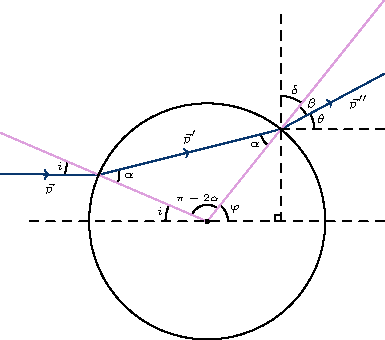
\includegraphics[width=0.5\textwidth]{figs/sphere.pdf}
    \end{center}
    \caption{Une sphère molle?}
    \label{fig: oui_une_sphere}
\end{figure}

\noindent

\question{a}{
    Premiere sous-question. Premiere sous-question. Premiere sous-question.
}

\fullindent

\blindduck[maths=both]

\rindent

\question{b}{
    Seconde sous-question. Seconde sous-question. Seconde sous-question.
}

\fullindent

\blindduck

\begin{align}
    \boxed{
        d = ra^k e.
    }
    \label{eq: test_1}
\end{align}

\rindent

\question{c}{
    Troisieme sous-question. Troisieme sous-question. Troisieme sous-question.
}

\fullindent

\blindtext

\rindent

\clearpage

